% ============================================================================
% 第 3 章 系统需求分析
% 预估页数：3 页
% 写作总要点：
%   - 围绕 "为什么要做这些功能" 展开，避免直接列功能清单
%   - 用例图、活动图等放在 figures/ 目录，引用 \ref{fig:xxx}
% ============================================================================
\chapter{系统需求分析}

% ----------------------------------------------------------------------------
\section{业务需求分析}

\subsection{医学问诊实训现状与痛点}
% 写作要点：
%   - 痛点 1：真实病例场景匮乏，标准化病人成本高
%   - 痛点 2：教师批量指导效率低，个性化反馈难
%   - 痛点 3：实训效果难以量化评估
%   - 痛点 4：学生缺乏 24/7 的反复练习机会

医学问诊训练要求学生在反复交流中熟悉病史采集、检查请求和初步诊疗思路。当前高校实训更多依赖课堂角色扮演或临床见习，训练次数和反馈深度都受师资、病例和时间限制。结合项目需求，本系统主要关注以下问题：

一是标准化病人资源不足。同学互相扮演病人时，表达和病情线索不够稳定；职业化标准化病人的培训与使用成本又较高。二是教师难以逐轮指导。一个教师通常要面对多个班级和大量训练报告，很难对每次问诊过程都给出细致点评。三是训练结果不易量化。传统评分多依赖主观判断，难以拆分到问诊、诊断、治疗和沟通等维度。四是学生课后缺少低成本的复练环境，无法随时围绕薄弱环节继续训练。

\subsection{用户角色分析}
% 写作要点：
%   - 学生：医学生 / 实习医生
%   - 教师：临床带教老师 / 班主任 / 教研室管理员（teacher\_admin）
%   - 管理员：系统管理员（admin / super\_admin）
%   - 用表格对比三个角色的核心需求

系统按使用职责划分为学生、教师和管理员三类使用面，并在权限实现中设置 \texttt{student}、\texttt{teacher}、\texttt{teacher\_admin}、\texttt{admin}、\texttt{super\_admin} 等角色键。学生关注病例训练和个人反馈；教师关注病例建设、训练过程查看与成绩批改；管理员负责用户、权限、日志和系统资源。表~\ref{tab:roles} 给出了三类角色的需求对比。

\begin{table}[H]
    \centering
    \caption{系统用户角色与核心需求对比}
    \label{tab:roles}
    \begin{tabular}{ll p{8cm}}
        \toprule
        角色 & 描述 & 核心需求 \\
        \midrule
        学生 & 医学生 / 实习生 & 选择病例开启问诊训练、进行多轮 AI 对话与临床检查、提交诊断与治疗方案、查看评分与能力雷达、复盘训练记录、查看个人薄弱点与趋势分析 \\
        教师 & 临床带教老师 / 教务管理员 & 创建与维护医学病例库、上传多媒体临床资料、管理班级与学生名单、查看学生 AI 问诊全过程、在 AI 评分基础上补充教师评分与评语、查看班级能力雷达与错误点分布 \\
        管理员 & 系统管理员 / 超级管理员 & 管理用户与角色、重置密码与冻结账号、查看系统运行状态与在线人数、审查操作日志与异常事件、维护存储与配置 \\
        \bottomrule
    \end{tabular}
\end{table}

% ----------------------------------------------------------------------------
\section{功能需求分析}

\subsection{学生端功能需求}
% 写作要点：
%   - AI 问诊训练（核心）
%   - 病例库浏览与详情
%   - 训练记录与报告
%   - 学习分析（雷达图、趋势图、薄弱点）
%   - 个人中心
%   - 强调："训练续接""智能推荐"等差异化功能

学生端以 AI 问诊训练为中心。训练由 \texttt{TrainingController} 和 \texttt{ChatController} 支撑，覆盖开始训练、多轮对话、检查结果调用、提交诊断与治疗方案、结束或放弃训练等流程。考虑到学生可能中途离开页面，系统还需要支持训练续接：重新进入未完成记录时，从 Memory 中恢复最近对话上下文。

除主流程外，学生端还包括病例浏览、训练记录、评估报告、学习分析和个人中心。病例库支持按科室、难度和关键词筛选；训练报告展示总分、四维能力、薄弱点和建议；学习分析接口 \texttt{/api/analysis/student} 提供能力雷达、成绩趋势和推荐病例。界面设计上，学生端应减少管理系统式表格堆叠，突出训练入口、对话反馈和复盘结果。

\subsection{教师端功能需求}
% 写作要点：
%   - 病例管理（创建 / 编辑 / 多媒体上传 / 发布 / 归档）
%   - 班级管理
%   - 成绩管理与批改工作台（教师评分 + AI 评分 + 教师评语）
%   - 教学分析（班级整体能力雷达、知识点错误统计）

教师端主要解决三件事：建设病例、查看训练过程、完成结果反馈。病例管理需支持创建、编辑、复制、发布和归档，并维护主诉、现病史、既往史、体格检查、辅助检查、参考诊断、治疗方案等字段。对于胸片、CT、超声、心电图和化验单等资料，系统需要提供附件上传和类型标注，方便后续临床工具匹配。

班级管理和训练记录查询用于过程监看：教师可以创建班级、添加学生、查看对话详情；跨班级、跨教师的数据访问仅开放给 \texttt{teacher\_admin} 以上角色。成绩与批改工作台由 \texttt{GradeController} 提供列表、详情、评分、统计和导出功能，教师可在 AI 评分基础上补充人工评语。\texttt{AnalysisController} 则提供班级雷达图和错误点分布，帮助教师发现共性问题。

\subsection{管理员端功能需求}
% 写作要点：
%   - 用户管理 / 角色管理 / 权限分配
%   - 系统监控 / 在线用户 / 接口性能
%   - 日志管理 / 操作日志审计
%   - 存储管理（MinIO 桶与配额）

管理员端负责系统运行与权限治理。用户管理需要支持查询、创建、修改、逻辑删除、重置密码、冻结与解冻；角色管理需要维护角色及其权限配置，并为菜单和接口级权限扩展预留字段。日志管理记录登录、写操作和异常信息，便于追踪问题。系统资源管理展示 CPU、内存、磁盘、在线用户数、业务数据量、MinIO 和 Redis 状态，为演示和日常维护提供依据。

\subsection{公共与核心技术需求}
% 写作要点：
%   - RBAC 权限控制（页面 / 菜单 / 按钮三级粒度）
%   - 文件上传与预览（医学影像）
%   - ECharts 数据可视化
%   - WebSocket / SSE 流式推送
%   - 邮件验证码、密码重置

公共能力包括认证授权、文件、可视化和 AI 流式响应。认证授权需支持验证码、登录失败锁定、密码重置、令牌刷新和 RBAC 权限控制；文件能力服务于医学影像、病例附件、头像和批改材料；可视化能力统一支撑学生复盘、教师统计和管理员监控；AI 流式响应基于 SSE 实现，避免长文本生成时页面长时间无反馈。

% ----------------------------------------------------------------------------
\section{非功能需求分析}

\subsection{性能需求}
% 写作要点：
%   - 系统响应时间 ≤ 2s
%   - AI 响应时间 ≤ 5s
%   - 支持 10000+ 并发（任务书指标）
%   - 影像文件上传与预览无卡顿

系统需兼顾普通业务接口、AI 对话和医学附件访问。一般查询和提交接口的响应时间控制在 2~秒以内，多表统计类接口控制在 5~秒以内；AI 请求重点关注首字返回时间，普通对话目标不超过 5~秒，包含 RAG 上下文拼接时目标不超过 8~秒。任务书要求支持 10000+ 在线用户，实际部署中需通过多实例、负载均衡和缓存实现。医学影像上传和预览则要求避免明显卡顿。表~\ref{tab:perf} 总结了关键性能指标。

\begin{table}[H]
    \centering
    \caption{系统关键性能指标}
    \label{tab:perf}
    \begin{tabular}{l l p{6cm}}
        \toprule
        指标维度 & 目标值 & 备注 \\
        \midrule
        一般接口响应时间 & $\le$ 2 秒 & 单表查询、列表分页、详情查询 \\
        重型查询响应时间 & $\le$ 5 秒 & 多表联合、班级统计、训练分析 \\
        AI 首字返回时间 & $\le$ 5 秒 & 不启用工具调用 \\
        AI RAG 首字返回时间 & $\le$ 8 秒 & 含知识检索与上下文拼接 \\
        并发在线用户 & $\ge$ 10000 & 任务书指标，以多实例部署为前提 \\
        附件上传大小上限 & $\le$ 50 MB & 医学影像与护理文档 \\
        \bottomrule
    \end{tabular}
\end{table}

\subsection{安全需求}
% 写作要点：
%   - 身份认证（JWT + 验证码 + 登录失败锁定）
%   - 权限控制（RBAC + 接口级防越权）
%   - 数据加密（敏感字段 AES）
%   - 防 SQL 注入、XSS、CSRF

医学教育系统包含学生身份信息、训练轨迹和成绩数据，安全需求不能只停留在登录校验。身份层面，密码采用 BCrypt 存储，登录结合验证码、JWT 和刷新令牌，并在连续失败后进行账号锁定。权限层面，前端路由、后端接口和业务数据范围需同时校验，尤其要防止学生查看他人记录、教师越权查看非本班数据。数据层面，系统预留 HTTPS、敏感字段加密和参数化查询能力；审计层面，登录、病例修改、评分和权限变更等操作需要写入日志。

\subsection{可用性与可维护性需求}
% 写作要点：
%   - 浏览器兼容（Chrome / Edge / Firefox / Safari）
%   - 桌面 + 平板 自适应
%   - 模块化设计、清晰的分包结构
%   - 日志完善、文档完整

可用性方面，前端需兼容 Chrome、Edge、Firefox 和 Safari 等主流浏览器，桌面端和常见平板分辨率下应保证问诊、批改和管理主流程可用。可维护性方面，后端按资源、业务、数据访问分层，前后端接口保持 REST 风格和统一响应体；项目需保留 \texttt{README}、初始化 SQL、Docker 部署说明和接口文档，便于后续交接。

% ----------------------------------------------------------------------------
\section{用例分析}
% 写作要点：
%   - 用一张总体用例图（figures/usecase\_overall.png）
%   - 选 1--2 个核心用例（如"完成一次 AI 问诊训练"）写用例规约
%   - 用例规约包括：用例名、参与者、前置条件、主要流程、扩展流程

图~\ref{fig:usecase_overall} 展示了三类主参与者与核心用例的关系。学生侧包括开始 AI 问诊训练、查看训练报告、查看学习分析和维护个人信息；教师侧包括创建与发布病例、管理班级、批改训练报告和查看教学分析；管理员侧包括用户与角色管理、系统监控和操作日志审查。身份认证、文件上传与预览、消息通知等作为公共能力被多个用例复用。

\begin{figure}[H]
    \centering
    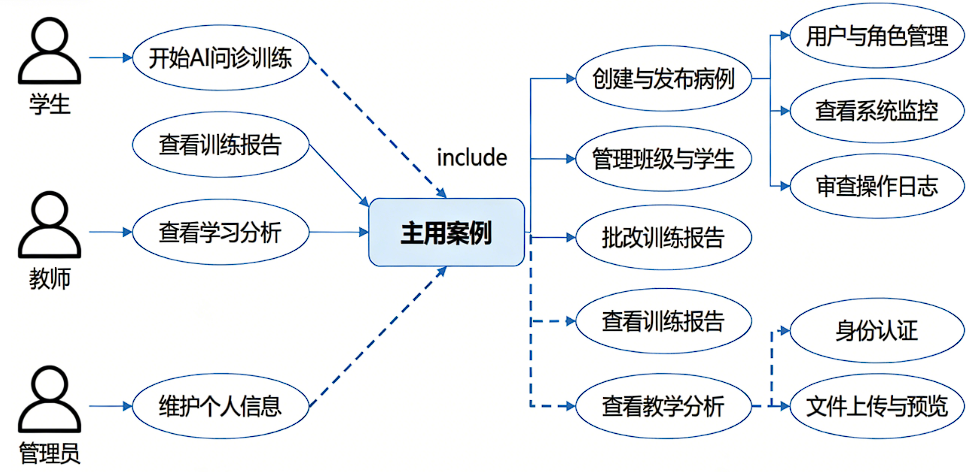
\includegraphics[width=0.85\textwidth]{figures/系统总体用例图.png}
    \caption{系统总体用例图}
    \label{fig:usecase_overall}
\end{figure}

本节选取“完成一次 AI 问诊训练”作为代表性用例，规约见表~\ref{tab:usecase}。该用例贯穿病例选择、Agent 对话、RAG、Memory、检查结果返回和评分生成，能够体现系统的主要业务链路。

\begin{table}[H]
    \centering
    \caption{用例规约：完成一次 AI 问诊训练}
    \label{tab:usecase}
    \begin{tabular}{l p{10cm}}
        \toprule
        项目 & 内容 \\
        \midrule
        用例名称 & 完成一次 AI 问诊训练 \\
        主参与者 & 学生 \\
        次参与者 & PatientAgent、DiagnosisAgent、FeedbackAgent、大语言模型服务 \\
        前置条件 & 学生已登录且账号状态正常，系统中至少存在一条已发布的病例 \\
        后置条件 & 生成一条训练记录与一条评分记录，并更新学生的学习分析指标 \\
        主流程 &
            (1) 选择病例“开始训练”；
            (2) 后端创建训练记录，返回记录 ID；
            (3) 学生输入问诊问题，前端以 SSE 调用接口；
            (4) 后端由 AgentRouter 选择 PatientAgent，从 Memory 与 RAG 中拼接上下文，调用大语言模型生成回复并以流式返回；
            (5) 学生可重复步骤 (3)～(4) 进行多轮问诊，然后提交诊断与治疗方案；
            (6) 生成多维评分与学习建议。 \\
        \bottomrule
    \end{tabular}
\end{table}

图~\ref{fig:activity_training} 进一步用 UML 活动图展示该训练流程。

\begin{figure}[H]
    \centering
    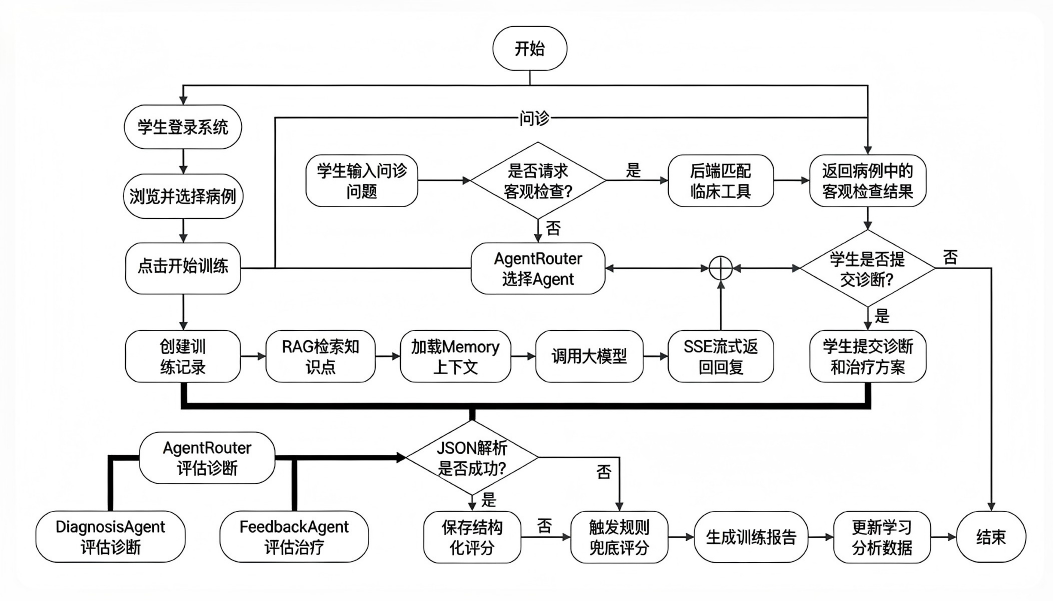
\includegraphics[width=0.75\textwidth]{figures/学生完成一次AI问诊训练活动图.png}
    \caption{学生完成一次 AI 问诊训练活动图}
    \label{fig:activity_training}
\end{figure}

% ----------------------------------------------------------------------------
\section{本章小结}

本章围绕问诊实训中的资源、反馈和评价问题，梳理了学生、教师和管理员三类角色的需求，明确了 AI 问诊训练、病例管理、学习分析、权限与运维等功能范围，并给出了性能、安全、可用性和可维护性指标。用例图与训练用例规约为后续架构设计提供了依据。
